\documentclass[tikz,border=6pt]{standalone}
\usepackage{amsmath,amssymb}
\usepackage{tikz}
\usetikzlibrary{arrows.meta}

\begin{document}
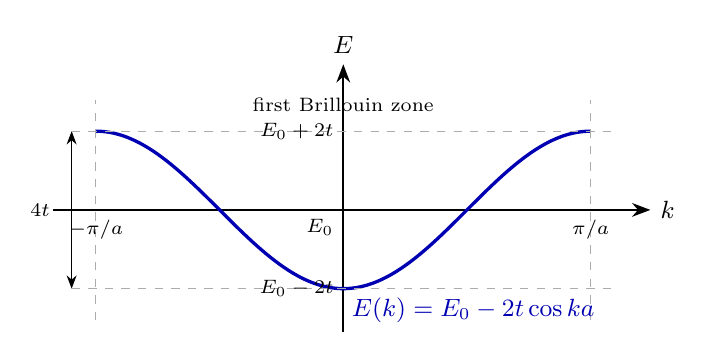
\begin{tikzpicture}[
    >=Stealth,
    axis/.style={->, thick},
    curve/.style={very thick, blue!70!black},
    guide/.style={dashed, gray!65},
    label/.style={font=\small},
    smalllabel/.style={font=\scriptsize}
]
    \draw[axis] (-3.7,0) -- (3.9,0) node[right, label] {$k$};
    \draw[axis] (0,-1.55) -- (0,1.85) node[above, label] {$E$};

    \draw[curve, domain=-3.14159:3.14159, samples=160]
        plot (\x,{ -cos(\x r) });

    \draw[guide] (-3.14159,-1.4) -- (-3.14159,1.4);
    \draw[guide] (3.14159,-1.4) -- (3.14159,1.4);
    \draw[guide] (-3.45,1) -- (3.45,1);
    \draw[guide] (-3.45,-1) -- (3.45,-1);

    \node[smalllabel, below] at (-3.14159,0) {$-\pi/a$};
    \node[smalllabel, below] at (3.14159,0) {$\pi/a$};
    \node[smalllabel, below left] at (0,0) {$E_0$};
    \node[smalllabel, left] at (0,1) {$E_0+2t$};
    \node[smalllabel, left] at (0,-1) {$E_0-2t$};
    \node[label, blue!70!black] at (1.65,-1.28) {$E(k)=E_0-2t\cos ka$};
    \draw[<->] (-3.45,1.0) -- (-3.45,-1.0);
    \node[smalllabel, fill=white, inner sep=1pt] at (-3.85,0) {$4t$};
    \node[smalllabel] at (0,1.33) {first Brillouin zone};
\end{tikzpicture}
\end{document}
